\subsection{Генерация карты перемещений}

На данной стадии с трассы собирается карта прав доступа для всех используемых приложением адресов. Далее производится слияние близких областей памяти с разрешенными комбинациями прав доступа. Максимальное расстояние для слияния областей является параметром командной строки. Затем производится перемещение полученных областей памяти в соответствии с новыми ограничениями адресации:

\begin{itemize}
    \item При наличии в исходной карте прав доступа областей с запрещенными комбинациями прав выводится ошибка -- корректное преобразование трассы невозможно.
    \item Области, при слиянии прав доступа которых получится комбинация прав, запрещенная новыми настройками адресации, размещаются на расстоянии, превышающем новый размер страниц памяти.
    \item Также перемещение производится только в области памяти, разрешенные новой конфигурацией.
\end{itemize}

Полученная карта перемещений используется последующими стадиями для анализа адресации и корректной замены адресов. Пример генерации карты перемещений приведен на рис. \ref{fig:reloc_map_example}.

\begin{figure}[h!]
    \centering
    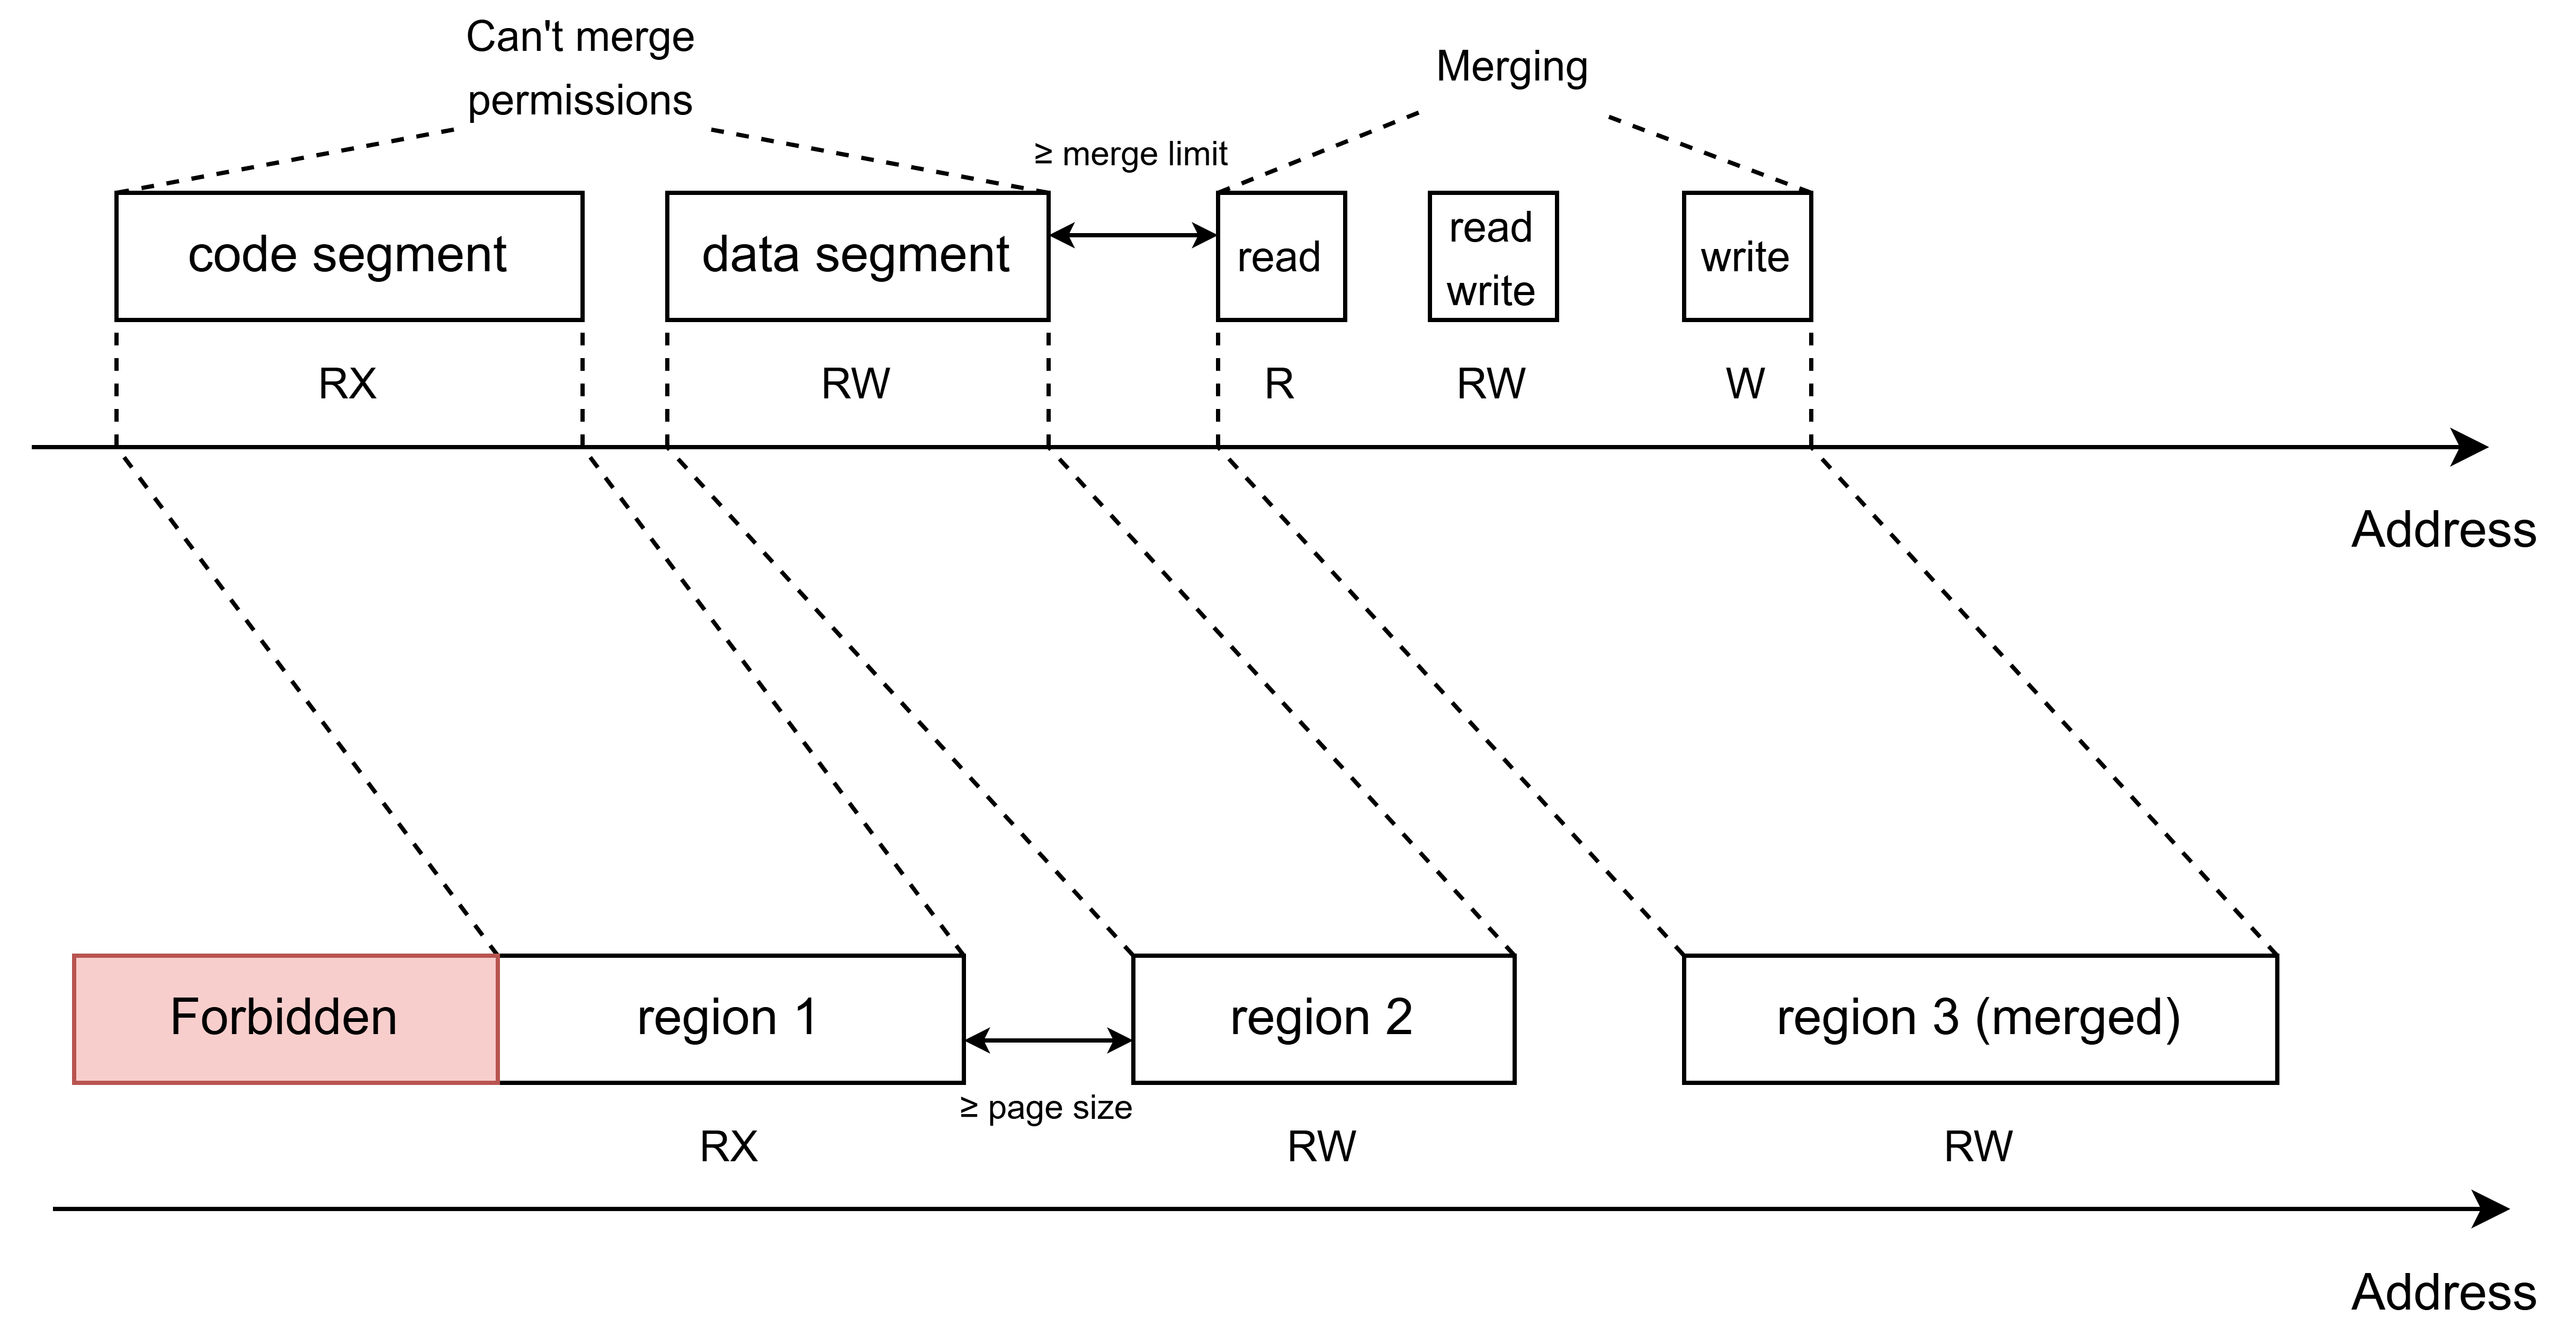
\includegraphics[width=0.9\linewidth]{pics/reloc_map_example.drawio.png}
    \caption{Пример генерации карты перемещений.}
    \label{fig:reloc_map_example}
\end{figure}

\FloatBarrier
